% Shared standalone design for the editable figure reconstructions.
\documentclass[tikz,border=5pt,10pt]{standalone}
\usepackage[T1]{fontenc}
\usepackage[utf8]{inputenc}
\usepackage{newpxtext,newpxmath}
\usepackage[scaled=.94]{sourcesanspro}
\usepackage{pgfplots}
\pgfplotsset{compat=1.18}
\usetikzlibrary{arrows.meta,calc,positioning,decorations.pathreplacing,
  decorations.markings,patterns,matrix,shapes.geometric,fit,backgrounds,
  intersections,angles,quotes}
\definecolor{ink}{HTML}{203746}
\definecolor{accent}{HTML}{146C78}
\definecolor{muted}{HTML}{667780}
\definecolor{signalred}{HTML}{B94B44}
\color{ink}
\tikzset{>=Latex,line width=.8pt,
  every node/.style={font=\small},
  axis/.style={->,draw=muted,line width=.5pt},
  guide/.style={draw=muted,dashed,line width=.45pt},
  curve/.style={draw=accent,line width=1pt},
  marker/.style={circle,fill=accent,inner sep=1.5pt},
  labelbox/.style={fill=white,inner sep=2pt}}

\begin{document}
\begin{tikzpicture}[x=1cm,y=1cm]
\foreach \shift/\title in {0/{$B_0$},3.9/{$B_1=B_0\star B_0$},7.8/{$B_2=B_1\star B_0$}} {
 \begin{scope}[shift={(\shift,0)}]
 \draw[axis] (-1.7,0)--(1.7,0) node[right] {$x$};
 \node at (0,2.2) {\title};
 \end{scope}}
\draw[curve] (-1.5,0)--(-.5,0)--(-.5,1.55)--(.5,1.55)--(.5,0)--(1.5,0);
\node[below] at (-.5,-.05) {$-\tfrac12$};\node[below] at (.5,-.05) {$\tfrac12$};
\draw[curve] (2.4,0)--(2.9,0)--(3.9,1.55)--(4.9,0)--(5.4,0);
\foreach \x/\lab in {2.9/-1,3.9/0,4.9/1} {\node[below] at (\x,-.05) {$\lab$};}
\begin{scope}[shift={(7.8,0)}]
\draw[curve,domain=-1.5:1.5,samples=121] plot (\x,{1.55*(abs(\x)<.5 ? .75-\x*\x : .5*(1.5-abs(\x))^2)});
\foreach \x/\lab in {-1.5/{-\tfrac32},0/0,1.5/{\tfrac32}} {\node[below] at (\x,-.05) {$\lab$};}
\end{scope}
\node at (3.9,-1.1) {$B_0=\mathbf{1}_{[-1/2,1/2]},\qquad B_m=B_0^{\star(m+1)}$};
\end{tikzpicture}
\end{document}
